% !TEX root = ../main.tex
% !TEX program = xelatex
\section{问题三的模型建立与求解}

\subsection{供需预测与动态准备}
新预报和当天观测有助于修正零点判断，但短时偏差未必持续，修改订单又需要付费。因此，本文采用\textbf{融合预测与日内校正滚动规划}：以同星期近期加权预测负载，用当天偏差修正后续需求；将官方光伏预报与近期历史融合，再由滚动规划权衡普通购电、改单和紧急补购费用。

光伏预测考虑直接使用官方预报、历史融合和提升树修正三种方法。历史融合能够结合当天预报与近期发电水平，权重含义清楚，实际费用比较也支持这一选择。

\subsubsection*{（1）兼顾星期规律与近期变化的负载预测}

负载保留问题二的同星期参照思路，但对较近的日期赋予更高权重。
设 $d$ 为当天，$k$ 为日内第 $k$ 个10分钟时段，零点负载预测为
\begin{equation}
\widehat L^{0}_{d,k}
=\sum_{j=1}^{4}\gamma_jL_{d-7j,k},\qquad
\gamma_j=\frac{0.5^{j-1}}{\sum_{i=1}^{4}0.5^{i-1}}.
\end{equation}
最近四个同星期日的权重依次为 $8/15$、$4/15$、$2/15$ 和 $1/15$。周权重按0.5逐周递减，使最近两周合计占80\%的权重，同时保留更早两周的信息。这样既突出近期用电变化，也保留同星期历史的参考作用。后文比较表明，该近期加权方案较四周等权方案费用更低。

\subsubsection*{（2）用当天已发生的负载修正后续判断}

用 $\tau\in\{0,36,72,108\}$ 表示决策时已经结束的时段数，
分别对应0:00、6:00、12:00和18:00。
在日内决策时，先计算当天已发生时段的平均负载偏差：
\begin{equation}
B_{d,\tau}=\frac{1}{\tau}\sum_{k=1}^{\tau}
\left(L_{d,k}-\widehat L^{0}_{d,k}\right),\qquad \tau>0.
\end{equation}
正偏差表示当天至今的用电高于预期，负偏差则表示低于预期。
随后，将尚未发生的时段按日内时刻划为3小时组，考察过去28个完整日中，
同一决策时刻的已发生偏差与各组后续偏差之间的关系。

设 $Y_{i,\tau,g}$ 为历史日期 $i$ 在未来第 $g$ 组的平均负载预测误差，
$\mathcal H_{d,\tau,g}$ 为可用历史日期集合，则修正系数为
\begin{equation}
\theta_{d,\tau,g}=\operatorname{clip}_{[0,1]}
\left(\frac{\sum_{i\in\mathcal H_{d,\tau,g}}B_{i,\tau}Y_{i,\tau,g}}
{\sum_{i\in\mathcal H_{d,\tau,g}}B_{i,\tau}^{2}}\right).
\end{equation}
该式是无截距最小二乘估计。当天没有偏差时不作额外修正；
历史上偏差延续得越明显，修正比例就越大。
将系数限制在0到1之间，可以避免反向修正或放大短时波动。
有效历史不足7天，或分母接近零时，取 $\theta_{d,\tau,g}=0$。

当天后续负载据此更新为
\begin{equation}
\widehat L_{d,k}^{\tau}
=\max\left\{0,\widehat L^{0}_{d,k}
+\theta_{d,\tau,g(k)}B_{d,\tau}\right\},\qquad k>\tau.
\end{equation}
系数只由此前完整日期估计，当前偏差只使用已经结束的时段。
零点不作日内偏差修正。次日的辅助负载预测仍由零点已知的同星期历史构造，不直接延续当天偏差。

\subsubsection*{（3）融合官方光伏预报与近期历史}

光伏与负载分别预测。附件3的官方预报按整点给出，本文先在整点融合官方预报与历史参考，
再转换为10分钟序列，以适应购电安排的时间尺度。

以 $\ell$ 表示预报所对应的整点，当前官方光伏预报为 $F_{d,\tau,\ell}$，
近期同钟点的历史参考为 $H_{d,\tau,\ell}$，则整点融合预测为
\begin{equation}
\widetilde P^{PV}_{d,\tau,\ell}
=\lambda_{d,\tau,h}F_{d,\tau,\ell}
+(1-\lambda_{d,\tau,h})H_{d,\tau,\ell}.
\end{equation}
历史参考取该钟点最近7次已结束时段的光伏均值。
这里的 $h$ 按预报提前1--6、7--12、13--18和19--24小时分组。
记 $\mathcal I_{d,\tau,h}$ 为过去28天中相同发布钟点、同一提前量组内已经兑现的样本集合，融合权重取为
\begin{equation}
\lambda_{d,\tau,h}
=\operatorname{clip}_{[0,1]}
\left(\frac{\sum_{i\in\mathcal I_{d,\tau,h}}(F_i-H_i)(P^{PV}_i-H_i)}
{\sum_{i\in\mathcal I_{d,\tau,h}}(F_i-H_i)^2}\right).
\end{equation}
该式选择使历史融合平方误差最小的比例，让两类信息相互补充。融合权重随发布时间和预测提前量变化，而不是全年固定不变。
同组样本不足24条时，合并相同发布钟点的其他提前量样本；仍不足24条，
或分母接近零时，取 $\lambda=1$，直接使用官方预报。

对融合后的相邻整点值作线性插值，得到10分钟光伏预测 $\widehat P^{PV}_{d,\tau,k}$。
决策时刚结束时段的光伏观测作为起点，尚未发生的真实光伏不参与计算。
当前预报只覆盖未来24小时，超过其覆盖范围至次日24:00的辅助时段，采用历史同钟点参考。

\subsubsection*{（4）根据近期净需求误差设置安全准备}

沿用第6.1节的净需求误差与加权分位方法，为可能低估的用电缺口设置准备。历史误差按原发布时间的预测计算，保证它反映当时能够形成的供需判断。

每次决策使用此前28天发布且已兑现的误差，按相同发布时间、目标日内3小时组，
以及预测距发布时间是否达到24小时分别归集。
历史误差仍按 $\omega_j\propto0.7^{a_j}$ 加权，$a_j$ 为相隔天数。28天窗口保留四周信息，3小时分组将每个6小时更新区间分成前后两段，使准备量兼顾近期变化和日内差异。
组内样本不足时合并相同发布时间和覆盖范围的误差，仍不足24条时不附加准备。

取加权误差的0.60分位，并将负值截为零，得到准备量
\begin{equation}
M_{d,\tau,k}=\max\left\{0,Q_{0.60}^{(\omega)}(\varepsilon)\right\}.
\end{equation}
0.60表示误差排序中的位置，不是多买60\%的电，也不是供电保证概率。
它与负载的周权重0.5、误差的日衰减0.7各有不同作用。
分位选得过低容易漏掉缺口，过高则增加无效订电；本问的分位比较见第7.6节。

\subsection{滚动购电模型与求解}

\subsubsection*{（1）供需关系与储能约束}

为简化表达，以下用 $t$ 连续编号当前时刻至次日24:00的时段，省略日期和发布时间下标。
考虑安全准备后的预计净需求为
\begin{equation}
N_t=(\widehat L_t-\widehat P^{PV}_t)\Delta t+M_t,\qquad
n_t=\max(N_t,0),\quad a_t=\max(-N_t,0).
\end{equation}
$N_t$ 为带符号的净需求，$n_t$ 为预计需要外网或电池补充的电量，$a_t$ 为预计可用于储能的光伏富余。
准备量只改变规划中的供需判断。沿用前文的订单、充放电与库存变量，另设预计紧急购电量 $e_t$ 和已订购但预计无法接收的电量 $u_t$，用于权衡改单、补购与订单过量的代价。



\noindent\textbf{约束1：计划供需平衡。}光伏优先直接满足负载后，其余供需满足
\begin{equation}
q_t-x_t+z_t+e_t-u_t=n_t.
\end{equation}
普通订单既能供负载，也能给电池充电。若订单有剩余且电池无法接收，
剩余部分计入 $u_t$，仍按订单付费。

\noindent\textbf{约束2：储能与供电范围限制。}功率、储电递推与容量限制沿用式\eqref{eq:q1_power_constraint}—\eqref{eq:q1_soc_bound}，另满足
\begin{equation}
0\le y_t\le a_t,\qquad z_t+e_t\le n_t,\qquad q_t,x_t,y_t,z_t,e_t,u_t\ge0.
\end{equation}
光伏充电不超过预计富余，电池放电和紧急补购不超过预计缺口。

\noindent\textbf{约束3：库存衔接与订单锁定。}每次从实际库存开始规划，日末余电传递至次日；已经执行的订单不再修改，仅优化剩余时段。

\subsubsection*{（2）订单调整费用}

设零点原始订单为 $q_t^0$，执行前最后确定的订单为 $q_t^F$。
按本文统一采用的结算口径，调减部分退回原计划电费，再收取原电价50\%的违约费；
调增部分支付电费及50\%的附加费。普通订单与调整费用合计为
\begin{equation}
C_{\mathrm{ord}}=\sum_t\left[p_tq_t^F+\frac12p_t|q_t^F-q_t^0|\right].
\end{equation}
例如，100~kWh订单在1元/kWh时减至80~kWh，结算为 $80+10=90$ 元。
同一时段多次调整，只比较最后订单与零点订单的净变化，重叠部分不重复收费。
该式也包含未能接收的普通订单费用，不能只按实际使用量结算。记$e_t^{\mathrm{act}}$为实际运行中电池仍无法补足的紧急购电量，则实际总费用为
\[
C_{\mathrm{act}}=C_{\mathrm{ord}}+5\sum_t p_t e_t^{\mathrm{act}},
\]
其中求和只覆盖实际执行的时段。它与规划中用于权衡风险的预计紧急购电量$e_t$不同，最终账单按实际补购计费。

\subsubsection*{（3）目标函数}

每次规划都延伸至次日24:00，使模型考虑留电对下一天的作用。
记 $\mathcal T_{\tau}$ 为全部规划时段，$\mathcal A_{\tau}$ 为其中当天尚未执行、
且已经在零点订过电的时段。零点决策时 $\mathcal A_0$ 为空。
目标函数为
\begin{equation}
\min J=\sum_{t\in\mathcal T_{\tau}}(p_tq_t+5p_te_t)
+\frac12\sum_{t\in\mathcal A_{\tau}}p_t\delta_t-\nu S_T,
\end{equation}
\noindent\textbf{辅助约束：调整量的线性化。}对 $t\in\mathcal A_{\tau}$，令
\begin{equation}
\delta_t\geq q_t-q_t^0,\qquad
\delta_t\geq q_t^0-q_t,\qquad\delta_t\geq0.
\end{equation}
只有当日已有订单的修改产生调整费。次日订单只是辅助规划，不在本次签订，也不收调整费。

末端库存系数取 $\nu=0.9p_{0:00}=0.38484$ 元/kWh，
以一度内部存电经放电后可替代的低价外网电作为参考。
$-\nu S_T$ 用于抑制规划末端放空电池的倾向，不是实际售电收入，不计入最终购电账单。
绝对值通过上述辅助变量转化为线性约束，采用HiGHS求解。

\subsubsection*{（4）滚动求解步骤}

\noindent\textbf{步骤1：制定零点原计划。}每天零点，读取已有历史、当前库存和官方预报，形成供需预测与准备量，求得并保存当天原始订单。次日的辅助安排仅用于判断当前应保留多少电。

\noindent\textbf{步骤2：执行购电与储能安排。}按第6.3节的实际供电规则运行至下一决策时点。光伏和普通电不足时由电池补充，剩余缺口紧急购买；余电在容量和充电功率允许时储存，并逐时更新实际库存。

\noindent\textbf{步骤3：利用新信息调整订单。}在6:00、12:00和18:00，更新负载偏差、光伏融合预测和准备量，从当前实际储电量重新求解。已经执行的订单锁定，未执行部分是否调整由费用权衡决定。随后继续执行步骤2，直至当天结束。

\noindent\textbf{步骤4：结算费用并衔接次日。}保留各时段执行前最后确定的订单，按照其相对零点订单的净变化计算调整费用，再加上实际紧急购电费。日末实际余电传递至下一天。

费用评价期为2025年2月1日至12月31日，共334天，起始库存沿用第6.3节的8592.69 kWh。各日连续运行，完整方案每天求解4次，共完成1336次滚动线性规划。

\subsection{候选方案比较}

为区分光伏预测方法的作用，先固定四周同星期等权负载、不作日内负载校正，
且不附加误差准备，只比较三种光伏处理方式。
各方案采用相同的设备、起始库存和结算规则，结果如表~\ref{tab:q3_candidate}所示。

\begin{table}[!htbp]
\centering
\caption{固定负载与准备条件下的光伏预测方案比较}
\label{tab:q3_candidate}
\begin{tabular}{lrrr}
\toprule
光伏处理方式 & 普通结算/万元 & 紧急购电/万元 & 总费用/万元\\
\midrule
直接采用官方预报 &1289.96&127.56&1417.51\\
历史误差融合预报 &1276.36&132.51&1408.87\\
提升树修正预报 &1279.46&136.80&1416.26\\
\bottomrule
\end{tabular}
\end{table}

历史融合降低的普通结算费用超过紧急购电费的增加，使总费用降至三种光伏方案中的最低水平。这说明官方预报与近期历史能够相互补充。在此基础上，引入误差准备，进一步处理低估缺口所带来的高价补购损失。

负载方面，在同样使用日内校正、融合光伏和0.60分位准备的条件下，
比较一周参照、两周等权、四周等权及四周近期加权，结果见表~\ref{tab:q3_load_compare}。
各方法均由自身的历史预测误差计算准备量，使准备程度与预测方法相匹配。

\begin{table}[!htbp]
\centering
\caption{同星期负载参照方式的费用比较}
\label{tab:q3_load_compare}
\begin{tabular}{lrr}
\toprule
负载参照方式 & 总费用/万元 & 紧急购电/万元\\
\midrule
最近一周 &1306.22&18.82\\
最近两周等权 &1303.74&17.85\\
最近四周等权 &1304.61&15.68\\
\textbf{最近四周近期加权} &\textbf{1301.42}&\textbf{16.13}\\
\bottomrule
\end{tabular}
\end{table}

四周近期加权保留较长历史以平滑单日异常，又能较快跟随近期用电变化。相较于四周等权，虽增加少量紧急购电费，但普通结算费用下降更多，最终节省约3.20万元。因此，本文选择近期加权，以获得更低的整体购电费用。两组比较分别支持历史融合与近期加权负载，二者共同用于本问的滚动规划。

\subsection{调度结果与分析}

\subsubsection*{（1）费用构成}

最终方案在334天内的普通订单费为1257.23万元，调整费为28.06万元，
二者合计普通结算费1285.29万元；紧急购电费为16.13万元。
总购电费用为\textbf{13014172.33元}。
评价期内紧急购电量为28627.32~kWh，共185天出现紧急购电。
评价期内未接收的普通订单为32.66万kWh，其费用已计入总支出。因此，需要同时权衡订电过量与紧急补购的代价。

\subsubsection*{（2）零点原计划与日内调整}

题目指定日期在0:00制定的部分购电计划见表~\ref{tab:q3_original_order}。
表中每项均为对应10分钟区间的电量，原计划在当天后续决策中保留，作为调整计费的基准。
% Generated from saved final Q3 trajectories. Do not hand-edit numbers.
\begin{table}[!htbp]
\centering
\caption{指定日期零点原计划的部分时段购电量（kWh）}
\label{tab:q3_original_order}
\small
\setlength{\tabcolsep}{5pt}
\begin{tabular}{lrrrr}
\toprule
时间段 & 3月20日 & 6月21日 & 9月23日 & 12月21日 \\
\midrule
10:00--10:10 & 0.00 & 0.00 & 0.00 & 0.00 \\
12:00--12:10 & 568.44 & 0.00 & 424.94 & 957.12 \\
14:00--14:10 & 0.00 & 0.00 & 0.00 & 0.00 \\
16:00--16:10 & 480.78 & 115.62 & 443.64 & 798.21 \\
18:00--18:10 & 722.54 & 426.86 & 810.48 & 727.22 \\
20:00--20:10 & 0.00 & 0.00 & 0.00 & 0.00 \\
\bottomrule
\end{tabular}
\end{table}


经过三次日内决策后，最终普通订单及全天费用见表~\ref{tab:q3_final_order}。
这里的最终订单是该区间执行前最后确定的总量，并非相对零点的增减量。6:00、12:00和18:00分别形成剩余时段的订单版本，已执行部分保持不变；各次版本用于追溯调整过程，最终订单用于实际结算。
零点计划与最终订单的差异反映了新供需判断和当前库存对后续安排的影响。
% Generated from saved final Q3 trajectories. Do not hand-edit numbers.
\begin{table}[!htbp]
\centering
\caption{指定日期调整后订单及全天费用（时段订单单位为kWh）}
\label{tab:q3_final_order}
\small
\setlength{\tabcolsep}{5pt}
\begin{tabular}{lrrrr}
\toprule
项目 & 3月20日 & 6月21日 & 9月23日 & 12月21日 \\
\midrule
10:00--10:10 & 0.00 & 0.00 & 0.00 & 0.00 \\
12:00--12:10 & 574.44 & 0.00 & 422.94 & 985.17 \\
14:00--14:10 & 0.00 & 0.00 & 0.00 & 0.00 \\
16:00--16:10 & 480.78 & 71.01 & 443.64 & 827.19 \\
18:00--18:10 & 722.54 & 415.06 & 810.48 & 727.30 \\
20:00--20:10 & 0.00 & 0.00 & 0.00 & 0.00 \\
\midrule
全天原计划购电量/kWh & 62950.87 & 40273.79 & 67565.05 & 94803.82 \\
全天最终普通订单/kWh & 62434.82 & 40006.24 & 67338.24 & 95848.96 \\
全天紧急购电量/kWh & 18.54 & 0.00 & 242.51 & 73.49 \\
普通结算费用/元 & 39514.95 & 22010.94 & 42247.91 & 62215.35 \\
紧急购电费用/元 & 117.15 & 0.00 & 1277.76 & 334.35 \\
全天总费用/元 & 39632.09 & 22010.94 & 43525.66 & 62549.70 \\
\bottomrule
\end{tabular}
\end{table}

前三个日期的最终订单低于零点计划，12月21日则增加约1045~kWh，
说明日内调整并非统一加量或减量，而是随供需判断变化。
表中各项分别四舍五入，费用合计由未舍入值计算。

\subsubsection*{（3）储能运行与紧急购电}

四个指定日期的实际充放电和日首尾库存见表~\ref{tab:q3_storage}。
充电量在电池输入侧计量，放电量在输出侧计量，首尾库存则为电池内部电量。
某个4小时区间同时有充电和放电，表示内部不同10分钟时段采取了不同动作，
不表示同一时段同时充放电。
% Generated from saved final Q3 trajectories. Do not hand-edit numbers.
\begin{table}[!htbp]
\centering
\caption{指定日期的实际充放电及日首尾储电量（kWh）}
\label{tab:q3_storage}
\small
\setlength{\tabcolsep}{5pt}
\begin{tabular}{llrrrr}
\toprule
时间段 & 项目 & 3月20日 & 6月21日 & 9月23日 & 12月21日 \\
\midrule
00:00--04:00 & 充电 & 1510.42 & 267.18 & 2048.71 & 1958.12 \\
 & 放电 & 238.58 & 302.32 & 61.89 & 239.38 \\
04:00--08:00 & 充电 & 1034.68 & 536.17 & 529.10 & 1617.46 \\
 & 放电 & 5467.56 & 1753.56 & 6328.62 & 793.91 \\
08:00--12:00 & 充电 & 4061.01 & 10134.27 & 4352.49 & 4419.79 \\
 & 放电 & 3259.44 & 0.00 & 2369.61 & 8608.93 \\
12:00--16:00 & 充电 & 6377.03 & 299.24 & 6833.50 & 8730.87 \\
 & 放电 & 254.72 & 0.00 & 417.27 & 2012.03 \\
16:00--20:00 & 充电 & 147.87 & 83.04 & 94.47 & 0.95 \\
 & 放电 & 4675.69 & 5205.83 & 5101.73 & 4983.07 \\
20:00--24:00 & 充电 & 4148.71 & 8559.86 & 8245.77 & 8334.82 \\
 & 放电 & 3749.74 & 3041.10 & 3620.94 & 3624.47 \\
\midrule
0:00 & 内部储电量 & 8871.16 & 2971.14 & 8609.68 & 8695.56 \\
24:00 & 内部储电量 & 4816.54 & 9415.36 & 8614.36 & 8738.25 \\
\bottomrule
\end{tabular}
\end{table}


指定日期发生紧急购电的时段见表~\ref{tab:q3_emergency}，未列出的时段为零。
6月21日没有紧急购电；其余日期的缺口也并非都由库存触底造成。
% Generated from saved trajectories by scripts/restore_review_tables.py.
\begin{table}[!htbp]
\centering
\caption{指定日期紧急购电的时段、电量及费用}
\label{tab:q3_emergency}
\small
\setlength{\tabcolsep}{5pt}
\begin{tabular}{llrr}
\toprule
日期 & 时间段 & 紧急购电量/kWh & 费用/元 \\
\midrule
3月20日 & 10:00--10:10 & 6.12 & 30.53 \\
 & 20:40--20:50 & 12.42 & 86.62 \\
6月21日 & 无 & 0.00 & 0.00 \\
9月23日 & 09:40--09:50 & 4.35 & 20.48 \\
 & 09:50--10:00 & 13.98 & 66.88 \\
 & 20:30--20:40 & 6.38 & 43.00 \\
 & 20:40--20:50 & 58.51 & 408.19 \\
 & 21:00--21:10 & 65.38 & 305.04 \\
 & 21:10--21:20 & 28.13 & 127.56 \\
 & 21:20--21:30 & 2.38 & 11.15 \\
 & 21:30--21:40 & 34.04 & 159.48 \\
 & 21:40--21:50 & 20.86 & 102.94 \\
 & 21:50--22:00 & 8.51 & 33.03 \\
12月21日 & 08:00--08:10 & 22.46 & 130.48 \\
 & 10:50--11:00 & 51.03 & 203.87 \\
\bottomrule
\end{tabular}
\end{table}


图~\ref{fig:q3_days}展示3月20日和9月23日的供需与储能过程。
3月20日两次补购均发生在电池降至最低库存时。
9月23日20:30，电池虽有余电，当段却已达到最大放电功率，仍需紧急补购；
随后多个时段又因库存触底而补购。

\begin{figure}[!htbp]
\centering
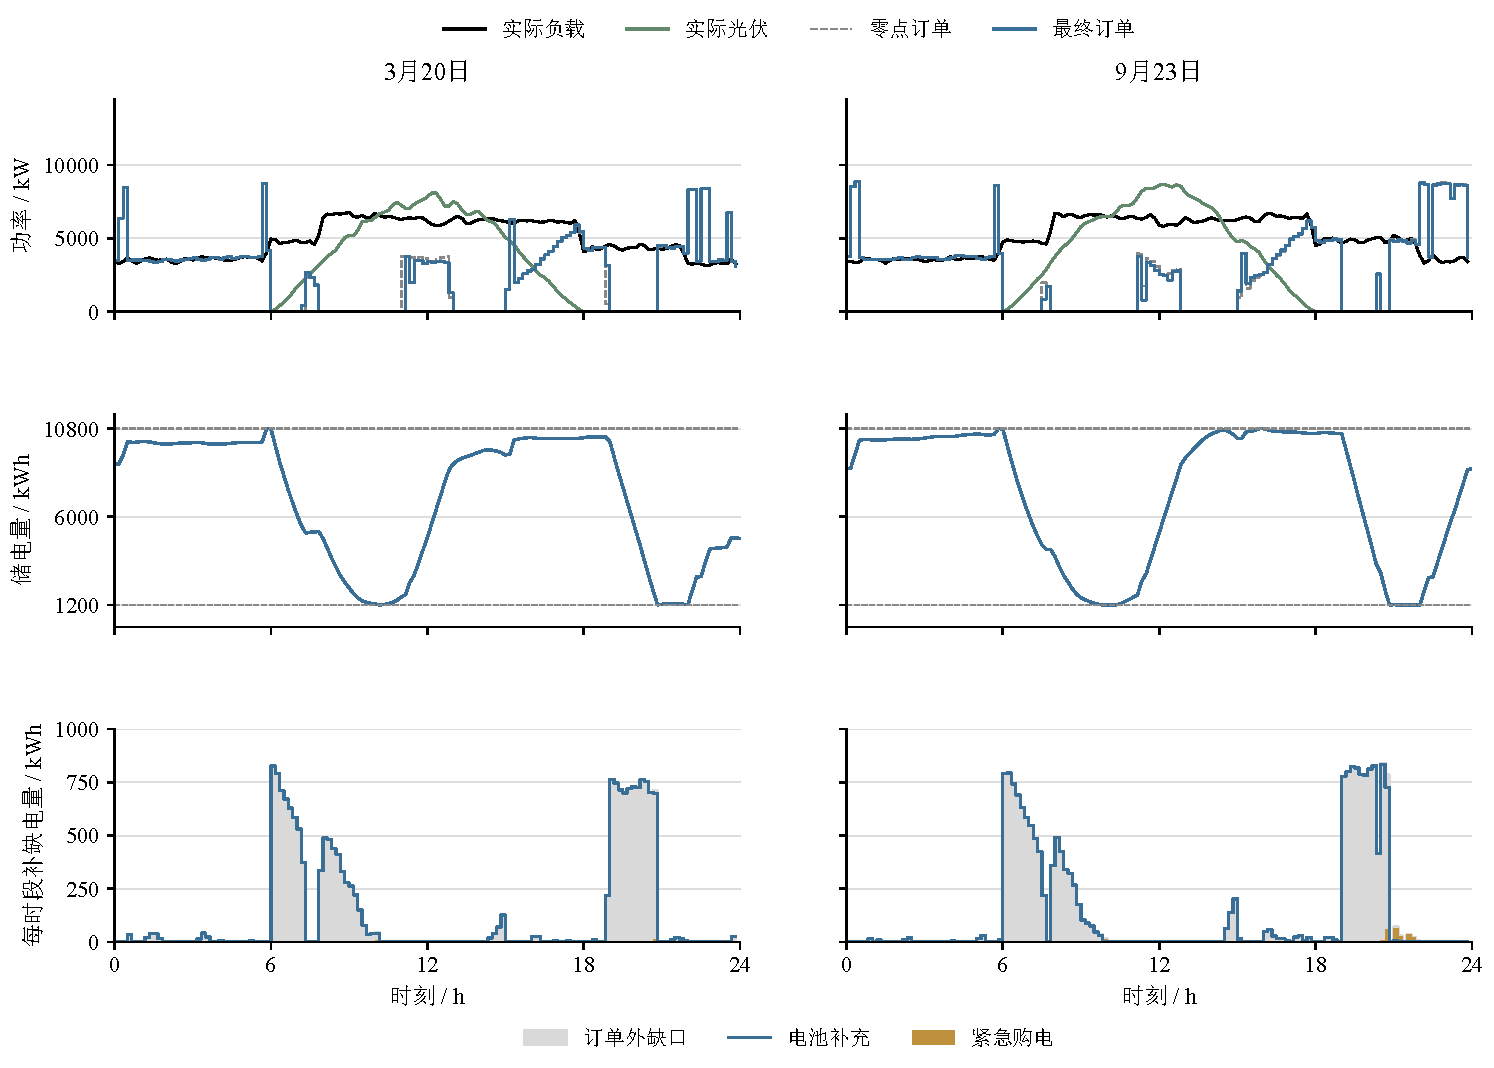
\includegraphics[width=0.88\textwidth]{fig/q3_final_days.pdf}
\caption{两个指定日期的供需、储电状态及缺口补充}
\label{fig:q3_days}
\end{figure}

这说明\textbf{库存下限和放电功率限制都可能触发紧急补购}，电池里有电并不等于任何时段都能及时供够。
判断紧急购电是否必要，必须同时考虑缺口出现的时刻、可用库存和放电功率，
不能只比较全天电量总和。

\subsection{日内新预报的价值}

为区分新预报与反馈改单各自的作用，本文在同一套负载预测、准备规则和调度结构下设置三组信息条件，共同从同一实际库存开始连续运行。第一组只在零点订电，全天不改单；第二组允许根据已发生的供需和库存调整，但不读取后发官方预报；第三组在第二组基础上加入后发官方预报。各组的预测误差与准备量均由自身可用信息构造，结果见表~\ref{tab:q3_info}。

\begin{table}[!htbp]
\centering
\caption{同一模型下三种信息条件的费用比较}
\label{tab:q3_info}
\begin{tabular}{lr}
\toprule
信息与决策条件 & 总费用/万元\\
\midrule
零点订电，全天不修改订单 &1359.00\\
日内反馈与改单，不使用后发官方预报 &1308.37\\
日内反馈与改单，使用后发官方预报 &1301.42\\
\bottomrule
\end{tabular}
\end{table}

日内反馈与改单使费用减少50.63万元。在此基础上，加入新光伏预报虽然增加调整费约6.86万元，但普通订单费和紧急电费分别减少约7.78万元、6.03万元，实现\textbf{6.95万元的净节省，降幅约0.53\%}。后两组期末库存相同，这部分收益并非靠多消耗剩余电量换来。

新预报还降低了对临时补购的依赖：紧急购电量由40956.71 kWh降至28627.32 kWh，\textbf{下降30.10\%}；紧急购电费下降27.22\%，出现紧急购电的日期由191天减少至185天。因此，新增调整支出换来了更大的购电节省，也减轻了临时高价补购的压力。

此外，未接收的普通订单由38.83万kWh降至32.66万kWh，\textbf{减少15.88\%}；未利用光伏电量减少3.07\%。这说明新预报有助于协调购电与储能，减少订多却用不上的电量，并促进光伏就地利用，符合绿色低碳发展的方向。

针对题目是否需要引入其他时刻预报的问题，本文认为，在给定条件下，\textbf{有必要将6:00、12:00和18:00发布的光伏预报纳入日内决策}。它们在已有反馈与改单能力的基础上，进一步降低费用、减少紧急补购和未利用电量。具体是否改单、调整多少，则由模型结合供需判断、储能余量与调整费用确定。

\subsection{参数检验}

为考察准备程度是否合适，保持负载与光伏预测、调度方式和结算规则不变，
将误差分位依次取0.40、0.50、0.60、0.70和0.80。
图~\ref{fig:q3_parameter}显示，总费用随准备程度先降后升，在五档比较中，0.60对应的总费用最低。

\begin{figure}[!htbp]
\centering
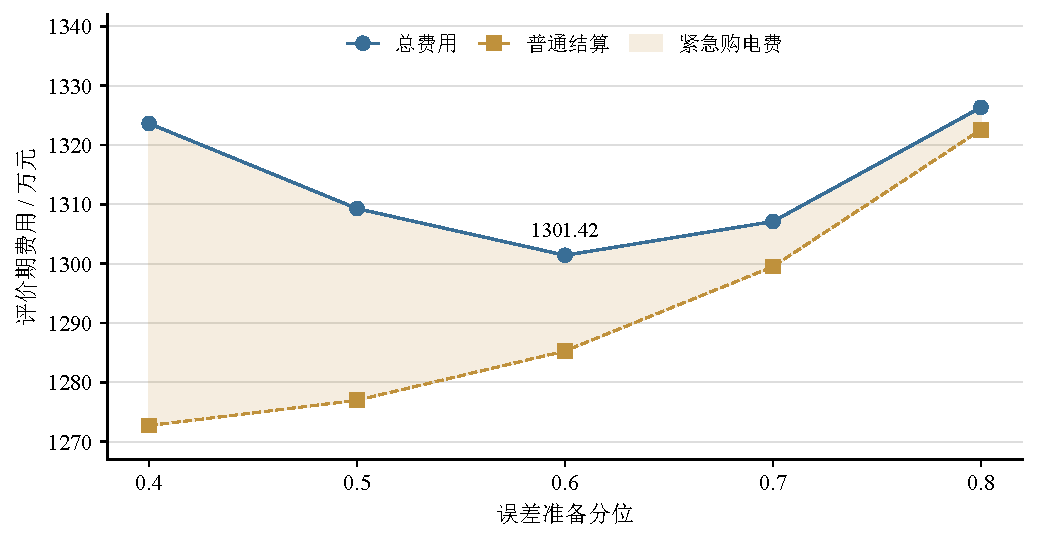
\includegraphics[width=0.64\textwidth]{fig/q3_final_quantile.pdf}
\caption{误差准备程度与购电费用的关系}
\label{fig:q3_parameter}
\end{figure}

准备不足会增加高价补购，准备过多又会增加普通订单及无法接收的电量。例如，分位从0.60提高到0.70后，紧急购电费减少约8.54万元，普通结算费却增加约14.23万元。因此，0.60在五档比较中较好地平衡了两类损失，体现了\textbf{适量准备对整体购电经济性的作用}。

计算后，逐10分钟核对供需平衡、库存衔接、充放电功率和已执行订单锁定，并由实际订单与紧急购电量重新计算账单。各项约束得到满足，费用复算差异小于0.01元。上述检验表明，方案在本文设定的信息与结算条件下能够连续执行，储能运行符合设备限制，购电费用可由实际订单逐项核算。
